\documentclass{llncs}

\usepackage{llncsdoc}
\usepackage{graphicx,url}
\usepackage[brazil]{babel}
\usepackage[utf8]{inputenc}
\usepackage{float}
\usepackage{setspace}

\usepackage{tabularx}
\usepackage{cite}
\usepackage{hyperref}

\begin{document}
\sloppy
\title{Pushing Together: A platform for social participation}

\author{Tallys Martins\inst{2}, Dylan Guedes\inst{2},
        Luan Guimarães\inst{2}, Paulo Meirelles\inst{1,2}}

\institute{Instituto de Matemática e Estatística -- Universidade de São Paulo (USP)\\
  Rua do Matão, 1010 -- 05508-090 -- Cidade Universitária -- São Paulo -- SP -- Brasil\\
  \email{\{diegoamc,manzo\}@ime.usp.br}
  \and
  Faculdade do Gama -- Universidade de Brasília (UnB)\\
  Gama -- DF -- Brasil\\
  \email{\{tallysmartins,djmgguedes,livreluan\}@gmail.com, paulormm@unb.br}}

\maketitle
\begin{abstract}
  % Contexto
  The brazilian government, as many others around the world, has been trying to
  build technologies for social participation in a collaborative way, exploring
  the guidance of the internet.
  % Problema
  Still, the participation process is more than just giving your opinion, it is
  also about dialog and discussion in a way we should have clear vision about all sides,
  all points of view, all kind of opinions, to discuss what is the best solution
  to a problem. However, the social networks and the recommendation systems, in their
  current design make a barrier in a way that we only receive content about
  what we like, about what we follow, about what our friends like. We are 
  stuck in bubbles of opinion.
  % Soluções propostas
  With this work we present Pushing Together, a free software platform
  for collaborative participation with the aim of breaking the bubbles that
  freezes people in their mindsets. The goal is to identify diferent groups of
  opinion in a conversation using clustering algorithms, and then give power to some
  special actors, bringing interaction between the groups.
  % Frase de impacto
  Through this project we hope to increase the engagement of people in terms of
  social participation and provide new resources for democracy processes.

\textbf{Keywords:} social participation, bubbles of opinion, democracy, gamification
\end{abstract}

\section{Introduction}
\label{sec:intro}
  Promoting social participation is a work made up of many challenges and can be
  analyzed from different aspects. Maybe the biggest one is to discover better
  ways of keeping the process in domain of both, laypeople and empowered ones,
  holding the engagement of the participants.

  Online discussions that happen in the standart ways, such as forums/threads, don’t
  provide an attractive dynamic for those who want to debate. Furthermore, it is
  impractical to do any deeper analysis with the generated information, for example,
  identify what are the opinion groups formed, or yet which opinion is majority
  or minority in discussions that occur in this molds. Natural language processing
  techniques would be extremely difficult to process this kind of information
  given the different themes and contexts of each conversation, outside the
  limitations in working with differents idioms.

  The Pushing Together project applies a different concept for the debates,
  called crowdsourced participation, which has shown to be a great option to break the
  the bariers for engagement and for opening more space to discussions. With little
  effort, the participants can give their opinion from small actions,
  something compared to a simple ‘like’ in a facebook comment.

  Composing people’s opinion in terms of agree and disagree, 0 or 1, it is possible
  to apply clustering algorithms to get sophisticated analysis of what people
  think about a subject in a discussion, and that is where we act.

  Analysing the opinion groups formed, we identify some profiles seen as special actors.
  Applying concepts of gamification we give power for those actors, allowing
  them to interact in the platform creating events and sending direct messages
  to others. With this strategy, we aim to change the communication and expression
  of opinion between different groups, facing what is known as bubbles of opinion,
  created by nowadays digital media.  

  %TODO criar um parágrafo explicando melhor as bolhas

\section{Related tools}

  There is a tool that was built on top of the crowdsourced participation concept.
  which served as inspiration for development of the Pushing Together project.
  The Polis\footnote{\url{https://pol.is}} is a web based platform that offers to
  users the possibility to create discussions about any subject. Then, people put
  140 characters comments demonstrating their point of view. The comments are
  presented to users as topics, on cards. The interaction on the system occur
  by others participants expressing their agreement or disagreement
  in existent comments, or yet by the addition of new ones to the conversation.

  Representing users opinions as vectors of 0 and 1, the Polis applies clustering algorithms
  that generates information about the groups of opinion formed, the most voted
  proposals and what proposals was agreed and disagreed by the most.

 \begin{figure}[H]
   \centering
   \begin{minipage}{.50\textwidth}
     \includegraphics[width=.9\linewidth]{images/polis1.png}
     \caption{Cards with comments}
     \label{fig:polis-2}
   \end{minipage}
   \begin{minipage}{.49\textwidth}
     \includegraphics[width=.9\linewidth]{images/polis2.png}
     \caption{Groups of opinion formed}
     \label{fig:polis-1}
   \end{minipage}
 \end{figure}

  As the Polis didn’t have the necessary resources for the development of
  the Pushing Together project, we had to implement them, like the identification of
  the special profiles inside the clusterization, support to mobile devices, a notification
  system and others more. The initial idea was to contribute and evolve Polis making it
  possible to achieve the new features. However, their community was not so
  open and we had many difficulties through this approach. The software was miss
  documented and we saw no transparency and support from the owners and maintainers.

  Given the barriers we’ve found, our tool was born with an independent
  architecture, encapsulating the Polis in a reverse engineering effort, waiting
  for it to evolve or, being more ambitious, aiming to develop our own clustering
  service. The second option demonstrated to be more tangible and was adopted to
  give sequence for the project.

\section{The Pushing Together project}
\label{sec:pushingtogether}

  The Pushing Together project was born in a kind of a Hackaton. An idea of the 
  brazilian NGO called Cidades Democráticas, which participated of an event
  called Collective Intelligence for Democracy, in Madrid, Spain at the end of
  the year 2016.

  With the goal of making the participation an easier process and breaking the
  bubbles of opinion, the project makes use of a resource that we named ‘the Push’,
  which is part of the gamification concept. Users in ownership of this 'power'
  will be able to send messages and create events inside the platform.

  Making an analysis about the users opinions in a conversation, we initially
  identify three profiles that are considered the potential receptors for the “Push”
  and some effects that can take place: 

 \begin{figure}[H]
   \centering
     \includegraphics[keepaspectratio=true,scale=0.25]{images/userprofiles.png}
   \caption{User profiles}
   \label{fig:userprofiles}
 \end{figure}


  With this initial shaping of the profiles we intend to get a different level
  of interaction between the multiple opinions in a group of discussion of a
  participative process. Although, this is still to be tested and validated for
  consolidation.

  From the technical aspects, the project is divided in a front end application,
  written in React Native, and a NodeJS server. The server module is responsible
  to manage users and the 'Push' resources in the gamification. Also, to make
  the interface with the external cluster processing service. All the communication,
  with the front end application and the cluster module, is made through an API. 
  The figure \ref{fig:architecture-2} below describes this architecture in general.

 \begin{figure}[H]
   \centering
     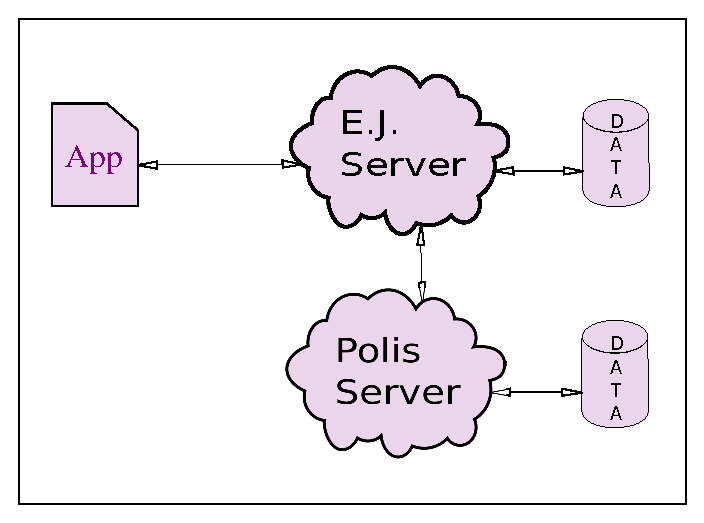
\includegraphics[keepaspectratio=true,,scale=0.5]{images/architecture-1.eps}
   \caption{Architecture of the system}
   \label{fig:architecture-2}
 \end{figure}

\section{Final remarks}
  The Pushing Together arise as a potential bridge for dialog between the society
  and the state, making a different analyzes about the opinion of the distinct
  groups and also opening new possibilities for the expression of these opinions
  with the ‘Push’ resource. Besides, the project was borns with transparence and
  colaboration principles, building a base for a prospective evolution.
\end{document}
